\documentclass{standalone}

\usepackage{tikz}
\usetikzlibrary{arrows,automata}
\usepackage{xcolor}
\definecolor{myblue}{RGB}{0,0,127} % navy blue


\begin{document}
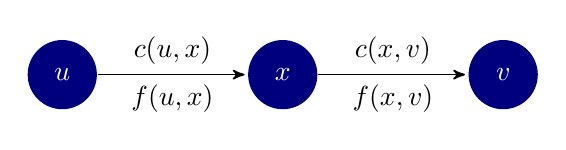
\begin{tikzpicture}[->,>=stealth',shorten >=1pt,auto,node distance=2.8cm, semithick]
  \tikzstyle{every state}=[fill=myblue,draw=none,text=white]

  \node[state]         (A)              {$u$};
  \node[state]         (B) [right of=A] {$x$};
  \node[state]         (C) [right of=B] {$v$};

  \path (A) edge              node[above] {$c(u,x)$} node[below] {$f(u,x)$} (B)
        (B) edge              node[above] {$c(x,v)$} node[below] {$f(x,v)$} (C);
\end{tikzpicture}
\end{document}
